%%% LaTeX Template
%%% This template is made for project reports
%%%	You may adjust it to your own needs/purposes
%%%
%%% Copyright: http://www.howtotex.com/
%%% Date: March 2011

%%% Preamble
\documentclass[paper=a4, fontsize=12pt]{scrartcl}	% Article class of KOMA-script with 12pt font and a4 format


\usepackage[english]{babel}				% English language/hyphenation
\usepackage[protrusion=true,expansion=true]{microtype}	% Better typography
\usepackage{amsmath,amsfonts,amsthm}			% Math packages
\usepackage[pdftex]{graphicx}				% Enable pdflatex
\usepackage{url}
\usepackage[margin=1.5in]{geometry}
\usepackage{algorithm}
\usepackage{algorithmic}
\usepackage{framed}
\usepackage{listings}

\lstset{
language=Matlab,
basicstyle=\footnotesize,
tabsize=2
}


%%% Custom sectioning (sectsty package)
\usepackage{sectsty}					% Custom sectioning (see below)
\allsectionsfont{\normalfont\scshape}			% Change font of al section commands


%%% Custom headers/footers (fancyhdr package)
\usepackage{fancyhdr}
\pagestyle{fancyplain}
\fancyhead{}						% No page header
%\fancyfoot[L]{\small \url{HowToTeX.com}}		% You may remove/edit this line 
\fancyfoot[C]{}						% Empty
\fancyfoot[R]{\thepage}					% Pagenumbering
\renewcommand{\headrulewidth}{0pt}			% Remove header underlines
\renewcommand{\footrulewidth}{0pt}			% Remove footer underlines
\setlength{\headheight}{13.6pt}


%%% Equation and float numbering
\numberwithin{equation}{section}		% Equationnumbering: section.eq#
\numberwithin{figure}{section}			% Figurenumbering: section.fig#
\numberwithin{table}{section}				% Tablenumbering: section.tab#


%%% Maketitle metadata (Defines how everything above the body should look like: title, header, authors, date, etc..)
\newcommand{\horrule}[1]{\rule{\linewidth}{#1}} 	% Horizontal rule

\title{
\vspace{-1in} 	
\usefont{OT1}{bch}{b}{n}
\normalfont \normalsize \textsc{University of Edinburgh - School of Informatics} \\ [25pt]
\horrule{0.5pt} \\[0.4cm]
\large IAR - Task 1 Report \\
\horrule{1pt} \\[0.5cm]
}
\author{
  \normalfont \normalsize
  Jakob Calero - s0948339\\[-3pt]\normalsize
  Samuel Neugber - s0821562\\[-3pt]\normalsize
  \today
}
\date{}


%%% Begin document
\begin{document}
\maketitle					% Insert the title here
\section{Abstract}
In a relatively static environment it may be possible to find all states a robot can be in and reduce them to conditions in the control code. This approach worked fine for our simple robot to do its simple task; it followed walls and avoided obstacles using a subsumption architecture based on the conditions we identified. A different approach we attempted to use was to directly inhibit the motor speeds using the information from the infra-red sensors. This resulted in smoother, but less predictable movement. Since the robot was more difficult to control using this method, we concentrated mainly on the conditional control to achieve the task.

\section{Introduction}
We approached the problem of navigating a small robot in a known environment using two different methods: Discrete, functional behaviour and more continuous, differential control, as described in the first few chapters of Vehicles\cite{vehicles}. The Khepera II robots are circular, two-wheeled robots, which come equipped with 8 infra-red sensors arranged as seen in \emph{figure 2.1}. 
\begin{figure}[!ht]
 \centering
  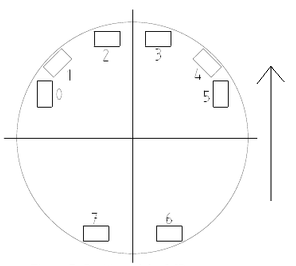
\includegraphics[width=0.5\textwidth]{IRSensors}
  \caption{Diagram of IR Sensors on Khepera robot}
\end{figure}

The goal was to move the robot around in a static and enclosed testing arena (\emph{figure 2.2}) while following walls and avoiding obstacles in unknown positions. The functional behaviour followed a simple subsumption control architecture, directly prioritising actions depending on conditional cases. The differential control on the other hand set the wheel speeds as a function of the values returned by the IR sensors. Both approaches were worked on simultaneusly and reviewed over time until one approach was chosen due to performing the task best.
\begin{figure}[!ht]
 \centering
  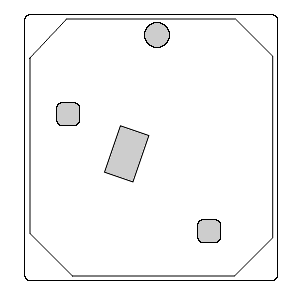
\includegraphics[width=0.75\textwidth]{mapexample}
  \caption{Map of driving area with example obstacle placements}
\end{figure}

\section{Methods}
\subsection{Gathering Data}
The IR sensors on the Khepera have a range of values between 0 and 1020. Experimentation showed that when nothing is close to the robot the sensor values drift at around 50. Sensor values of 200+ describe a sensible value representing the robot being near an object (within 2cm) while values of 500+ mean that we are too close to an object. A range between 180 and 250 where the values we chose as a good distance when trying to follow a wall without getting too close or too far away from it. From these values we then extrapolated if necessary.
\subsection{Functional Control}
As seen in \emph{figure 3.1} our control code for this methodology uses just four if-statements.

\begin{figure}[!ht]
\begin{framed}
\begin{algorithmic}
 \IF{FrontSensor is close to object \textbf{OR} RightSensors are close to object}
 \STATE{Command: Rotate left}
 \ENDIF
 \IF{FrontSensor is close to object \textbf{OR} LeftSensors are close to object}
 \STATE{Command: Rotate right}
 \ENDIF
 \IF{LeftSensor is closer than 250 but further away than 180 from object}
 \STATE{Command: Rotate left}
 \ENDIF
 \IF{RightSensor is closer than 250 but further away than 180 from object}
 \STATE{Command: Rotate right}
 \ENDIF
 \STATE{Command: Move forward}
\end{algorithmic}
\end{framed}
\caption{Functional Control Algorithm}
\end{figure}

Given the order each condition is checked the robot will always turn whenever there is something directly in front of the it, as illustrated by the first two conditions above. In the same two conditions the right and left sensors are also checked but only for a very close distance, triggering only when collision is imminent and not while travelling along a wall. These two simple cases result in the behaviour of avoiding object collision and the tendency of following straight objects (walls) given that as soon as the front sensor is not detecting anything forward movement is resumed.

The final two conditions attempt to capture the fact that the robot may turn away from a wall too much when avoiding collision or drift slightly. The robot should rotate back towards the wall if it has moved too far away. A cap to that distance is used as we do not want the robot to start rotating when it's \emph{very} far away from a wall as that might indicate it's not following a wall to begin with.
\subsection{Differential Control}
The second approach we took to solve the task ahead was one described in the first few chapters of Vehicles\cite{vehicles}. Our goal was that, ideally, the robot should always be moving and do so as smoothly as possible to maximise efficiency and avoid ``stuttering'' movement. The control code in \emph{Appendix 6.2} shows that in order to do so, each iteration of the control loop resets the wheel speed to a maximum value and then reduces the speed of the wheel on the opposite side of the corresponding IR sensor if certain thresholds are met. The higher the value of the sensor, the more the speed of the corresponding wheel is reduced.
\section{Results}
\subsection{Functional Control}
Using functional control, the behaviour of the robot was close to being deterministic, reliably following walls with 1-2cm distance. It managed to avoid obstacles to avoid collision and return to the wall searching pattern immediately after.

A few problems still remain however. One case was that it got stuck in narrow passages, such that the first two rules in the control loop were repeatedly activated in succession. An additional case where the robot would not explore the entire map if objects were placed in a square-like pattern, resulting in the robot moving in a loop between the objects without being able to get out.
\subsection{Differential Control}
Differential control did not work as intended in most cases, so we did not pursue it for long. The robot did turn smoother than it had using functional control, but it was also harder to control. The robot usually turned away too much when avoiding collision, which meant that it rarely followed a wall. This method did however have the benefit that the robot did not get stuck in between even the closest gaps, but nicely navigated through.
\section{Discussion}
In an environment as small and predictable as the one given in this task, good rule based behaviour is possible since most conditions the robot can be extracted and mapped accordingly and good results follow therein, as shown above. However, the more complex the task and environment get, the harder it will be to achieve such a design. In these cases, differential control, (or even better, full proportional–integral–derivative control) and more dynamic basic behaviour will be useful. Conditional if-cases will run into problems like the \emph{indecisiveness} of our above problem when navigating narrow corridors and are generally very messy to maintain.
\section{Appendix}
\subsection{Functional Controller - Source}
\lstinputlisting{controlMain.m}
\subsection{Differential Controller - Source}
\lstinputlisting{controlAlternate.m}
\begin{thebibliography}{9}
\bibitem{vehicles}
  Valentino Braitenberg,
  \emph{Vehicles: Experiments in Synthetic Psychology},
  A Bradford Book,
  1986.
\end{thebibliography}

%%% End document
\end{document}
